% BÀI TOÁN HÌNH HỌC - BAI_HINH_10 (TRÍCH ĐỀ 10)
\begin{ex}
% Câu 13
	Cho đường tròn $(O;R)$ và đường thẳng $d$ không đi qua $O$ cắt $(O)$ tại hai điểm $A; B$. Trên tia đối của tia $BA$ lấy điểm $M$; qua $M$ kẻ hai tiếp tuyến $MC; MD$ với đường tròn $(O)$ ($C; D$ là các tiếp điểm). Gọi $H$ là trung điểm của $AB$.
	\begin{enumerate}
		\item[a)] Chứng minh tứ giác $OMCH$ nội tiếp.
		\item[b)] $OM$ cắt $CD$ tại $K$. Đường thẳng qua $O$ vuông góc với $OM$, cắt tia $MC$ và $MD$ lần lượt tại $P$ và $Q$. Chứng minh $OK \cdot OM = R^2$ và tính độ dài $OM$ theo $R$ sao cho diện tích tam giác $MPQ$ nhỏ nhất.
	\end{enumerate}
\loigiai{
{
		\begin{center}
			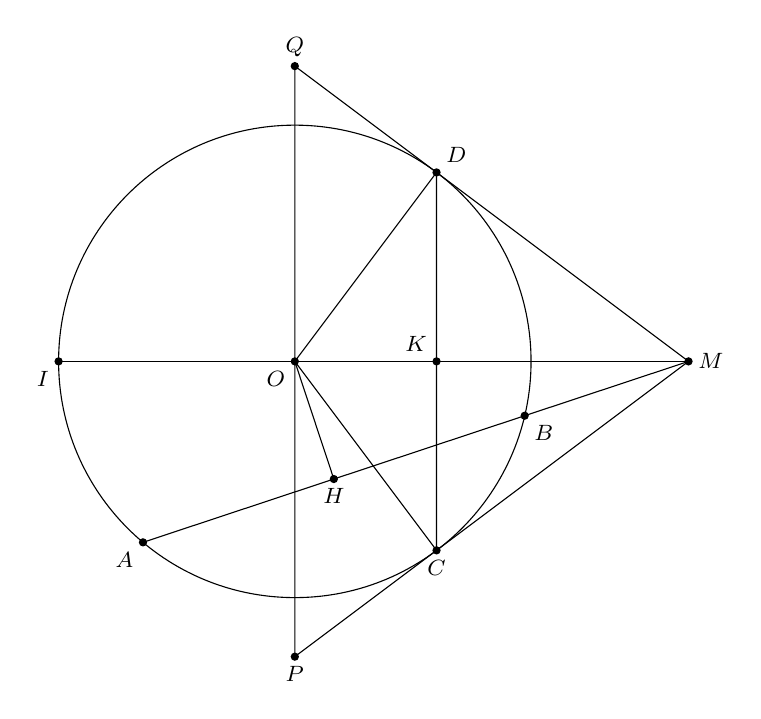
\begin{tikzpicture}[line join = round, line cap=round,>=stealth,font=\footnotesize,scale=1]
				\usetikzlibrary{calc}
				
				% Khai báo các giá trị cơ bản
				\def\r{3}
				\def\a{5}
				% acos trong pgfmath trả về giá trị bằng độ, phù hợp cho tọa độ cực của TikZ
				\pgfmathsetmacro{\alphaVal}{acos(\r/\a)}
				\pgfmathsetmacro{\kVal}{sqrt(\a*\a*\r*\r/(\a*\a-\r*\r))}
				
				% Định nghĩa tọa độ các điểm
				\coordinate (O) at (0,0);
				\coordinate (I) at (-\r,0);
				\coordinate (M) at (\a,0);
				\coordinate (D) at (\alphaVal:\r);      % D theo tọa độ cực (góc alphaVal, bán kính r)
				\coordinate (C) at (-\alphaVal:\r);     % C theo tọa độ cực (góc -alphaVal, bán kính r)
				\coordinate (Q) at (0, \kVal);        % Q(0,k)
				\coordinate (P) at (0, -\kVal);       % P(0,-k) - giả định từ Q(0,k) thứ hai
				\coordinate (A) at (-130:\r);         % A theo tọa độ cực
				
				% Các điểm được tính toán
				\coordinate (H) at ($(A)!(O)!(M)$);    % H là hình chiếu của O lên AM
				\coordinate (B) at ($2*(H)-(A)$);    % B sao cho H là trung điểm AB
				\coordinate (K) at ($(D)!0.5!(C)$);    % K là trung điểm DC
				
				% Vẽ các đối tượng hình học
				\draw (O) circle (\r);              % Đường tròn (O,r)
				\draw (P) -- (Q) -- (M) -- cycle;   % Tam giác PQM
				\draw (O) -- (D) -- (C) -- cycle;   % Tam giác ODC
				\draw (I) -- (M);                   % Đoạn thẳng IM
				\draw (M) -- (A);                   % Đoạn thẳng MA
				\draw (H) -- (O);                   % Đoạn thẳng HC
				
				% Tô màu và đặt nhãn cho các điểm
				\fill (O) circle (1.5pt);
				\fill (B) circle (1.5pt);
				\fill (I) circle (1.5pt);
				\fill (D) circle (1.5pt);
				\fill (C) circle (1.5pt);
				\fill (Q) circle (1.5pt);
				\fill (P) circle (1.5pt);
				\fill (A) circle (1.5pt);
				\fill (M) circle (1.5pt);
				\fill (H) circle (1.5pt);
				\fill (K) circle (1.5pt);
				
				\node[below left] at (O) {$O$};
				\node[below left] at (A) {$A$};
				\node[below right] at (B) {$B$};
				\node[below left] at (I) {$I$};
				\node[above right] at (D) {$D$};
				\node[below] at (C) {$C$};
				\node[above] at (Q) {$Q$};
				\node[below] at (P) {$P$};
				\node[right] at (M) {$M$};
				\node[below] at (H) {$H$};
				\node[above left] at (K) {$K$};
				
			\end{tikzpicture}
			
		\end{center}
		
		OM cắt CD tại K. Chứng minh $OK \cdot OM = R^2$. \\
		\\
		Ta có: Tam giác $ODM$ vuông tại $D$ (vì $\widehat{ODM} = 90^\circ$). \\
		Mặt khác: $MC = MD$ (Tính chất hai tiếp tuyến cắt nhau); \\
		$OC = OD = R$. \\
		Suy ra $OM$ là đường trung trực của đoạn thẳng $CD$ suy ra $OM \perp CD$. \\
		\\
		Trong tam giác vuông $ODM$ tại $D$ và tam giác $OKD$ đồng dạng (g-g) nên ta có: \\
		$OD^2 = OK \cdot OM$. \\
		suy ra $OK \cdot OM = R^2$. \\
		\\
		Theo t/c hai tiếp tuyến cắt nhau ta có $MO$ là tia phân giác của góc $PMQ$, mặt \\
		khác $MO \perp PQ$ nên tam giác $PMQ$ cân tại $M$ suy ra $PQ = 2OP$. \\
		\\
		Ta có $S_{PMQ} = \frac{1}{2} MO \cdot PQ = MO \cdot OP$. \\
		\\
		Trong tam giác vuông $OMP$ ta có: $OC \cdot PM = OP \cdot OM$. \\
		$\Rightarrow OC^2 \cdot PM^2 = OP^2 \cdot OM^2$ \\
		\\
		$\frac{1}{OC^2} = \frac{1}{OP^2} + \frac{1}{OM^2}$ suy ra $\frac{1}{R^2} = \frac{1}{OP^2} + \frac{1}{OM^2}$. \\
		\\
		Áp dụng bất đẳng thức Cô si : \\
		$\frac{1}{OP^2} + \frac{1}{OM^2} \ge 2 \sqrt{\frac{1}{OP^2} \cdot \frac{1}{OM^2}} = \frac{2}{OP \cdot OM}$ suy ra $\frac{1}{R^2} \ge \frac{2}{S_{PMQ}}$. \\
		\\
		$S_{PMQ} \ge 2R^2$. Dấu “=” xảy ra khi
		$\begin{cases}
			\frac{1}{OP^2} = \frac{1}{OM^2} \\
			OM \cdot OP = 2R^2
		\end{cases}$
		suy ra $OM = OP = R\sqrt{2}$. \\
		\\
		Vậy $S_{PMQ}$ đạt giá trị nhỏ nhất khi $OM = R\sqrt{2}$.
}
\end{ex}
